% Slide họp trao đổi với Giảng viên phản biện — HSGE.
% Bản ngắn, tách riêng khỏi slide bảo vệ (Slide_KLTN_HSGE); dùng chung theme
% và hình vẽ của slide bảo vệ.
% Build: latexmk -pdf main.tex   (pdflatex, tiếng Việt qua T5 fontenc)
% Preamble: document class, theme, Vietnamese support, shared macros.
% Same look-and-feel as Slide_KLTN_HSGE (defense deck); this deck is the
% shorter, working-meeting version for the phản biện.
\documentclass[aspectratio=169]{beamer}

\usetheme{Antibes}
\usecolortheme{whale}

% Vietnamese: T5 encoding (vntex) + Latin Modern covers the beamer sans family.
\usepackage[utf8]{inputenc}
\usepackage[T5]{fontenc}
\usepackage{lmodern}
\usepackage{textcomp}

\usepackage{graphicx}
\usepackage{booktabs}
\usepackage{array}
\usepackage{xcolor}
% Reuse the figures already built for the defense deck instead of duplicating them.
\graphicspath{{images/}{../Slide_KLTN_HSGE/images/}}

\usepackage{etoolbox}

% Navigation symbols & clean headline showing current section & subsection
\setbeamertemplate{navigation symbols}{}
\setbeamertemplate{mini frames}{}
\setbeamertemplate{headline}{%
  \leavevmode%
  \ifstrempty{\insertsectionhead}{}{%
    \begin{beamercolorbox}[wd=\paperwidth,ht=2.5ex,dp=1.1ex,leftskip=1.2em,rightskip=1.2em]{section in head/foot}%
      \usebeamerfont{section in head/foot}\scriptsize\textbf{\insertsectionhead}%
      \ifstrempty{\insertsubsectionhead}{}{%
        {\color{structure.fg!40}\ \textbf{|}\ }\normalfont\textit{\insertsubsectionhead}%
      }%
    \end{beamercolorbox}%
  }%
}

% A clean footline: reserves a bottom margin and gives slide numbers (without author)
\setbeamertemplate{footline}{%
  \hbox{\begin{beamercolorbox}[wd=\paperwidth,ht=2.2ex,dp=1.0ex,leftskip=1.2em,rightskip=1.2em]{section in head/foot}%
    \hfill\usebeamerfont{footline}\scriptsize\insertframenumber\,/\,\inserttotalframenumber%
  \end{beamercolorbox}}%
}

\setbeamertemplate{caption}[numbered]
\setbeamercolor{block title}{bg=structure.fg!15,fg=black}
\setbeamercolor{block body}{bg=structure.fg!5}

% Harvey balls for the positioning table (same notation as the thesis / defense deck).
\usepackage[nointegrals]{wasysym}

% Fixed-width column types reused by the result tables.
\newcolumntype{L}[1]{>{\raggedright\arraybackslash}p{#1}}
\newcolumntype{C}[1]{>{\centering\arraybackslash}p{#1}}
\newcolumntype{R}[1]{>{\raggedleft\arraybackslash}p{#1}}

% Caption line under a figure on a slide.
\newcommand{\figcap}[1]{\vspace{0.1cm}{\scriptsize\itshape #1}}

% Highlight for the key number of a slide.
\newcommand{\kw}[1]{\textbf{\color{structure.fg}#1}}

\title[HSGE --- Trao đổi phản biện]{Buổi trao đổi với Giảng viên phản biện}
\subtitle{HSGE --- Hierarchical Skill-Graph Exploration}

\author[Bảo Kiệt --- Tiến Phát]{
  \texorpdfstring{Trương Bảo Kiệt --- 22127223 \\ Hồ Tiến Phát --- 22127321}{Trương Bảo Kiệt, Hồ Tiến Phát}
}

\institute[HCMUS]{
  Giảng viên hướng dẫn: PGS.TS. Nguyễn Văn Vũ \\[0.2cm]
  \small Bộ môn Công nghệ Phần mềm \\
  Khoa Công nghệ Thông tin --- Trường Đại học Khoa học Tự nhiên, ĐHQG-HCM
}

\date{Khóa luận tốt nghiệp --- 2026}


\begin{document}

\begin{frame}[plain]
  \titlepage
\end{frame}

% Outline frame — chỉ 3 mục, một cột là đủ.
\begin{frame}{Nội dung buổi trao đổi}
  \small
  \tableofcontents
\end{frame}

% Show outline before each section
\AtBeginSection[]
{
  \begin{frame}{Nội dung buổi trao đổi}
    \small
    \tableofcontents[currentsection]
  \end{frame}
}

% !TEX root = ../main.tex

%%% ============================================================
\section{Động lực và nền tảng bài toán}
%%% ============================================================

\begin{frame}{Động lực, bài toán và định vị nghiên cứu}
  \begin{columns}[t]
    \begin{column}{0.48\textwidth}
      \footnotesize
      \textbf{Động lực}
      \begin{itemize}\setlength{\itemsep}{2pt}
        \item \textbf{Web Agent \& LLM lớn}: phụ thuộc API đám mây $\rightarrow$ chi phí cao, độ trễ lớn, rủi ro riêng tư.
        \item \textbf{SLM ($<10$B)}: chạy cục bộ, chi phí thấp $\rightarrow$ cần fine-tune để chuyên biệt hóa.
        \item \kw{Nút thắt dữ liệu}: gán nhãn thủ công tốn kém (AutoWebGLM: \textbf{20 người $\times$ 1 tháng}); dữ liệu tổng hợp giảm $\approx$\textbf{97\%} chi phí/mẫu (Synatra).
      \end{itemize}

      \vspace{0.1cm}
      \begin{block}{Phát biểu bài toán}
        \footnotesize
        Tự động khám phá website đang hoạt động và tinh chỉnh SLM hoàn thành task ngôn ngữ tự nhiên \textbf{không dùng dữ liệu do con người gán nhãn}.
      \end{block}
    \end{column}
    \begin{column}{0.50\textwidth}
      \footnotesize
      \textbf{Định vị so với công trình liên quan}
      \vspace{0.05cm}

      \scriptsize
      \setlength{\tabcolsep}{2.5pt}
      \begin{table}
        \begin{tabular}{@{}L{1.9cm} C{1.0cm} C{1.05cm} C{1.05cm} C{1.0cm}@{}}
          \toprule
          \textbf{Hệ thống} & \textbf{Khám phá} & \textbf{Skill kiểm chứng} & \textbf{Ghép task dài} & \textbf{Huấn luyện SLM} \\
          \midrule
          AWM & - & \LEFTcircle & - & - \\
          SkillWeaver & - & \CIRCLE & \LEFTcircle & - \\
          NNetNav & - & - & - & \CIRCLE \\
          Go-Browse & \CIRCLE & - & - & \CIRCLE \\
          \textbf{HSGE} & \CIRCLE & \CIRCLE & \CIRCLE & \CIRCLE \\
          \bottomrule
        \end{tabular}
      \end{table}
      {\scriptsize \CIRCLE{} Có \quad \LEFTcircle{} Một phần \quad - Không.}

      \vspace{0.08cm}
      \textbf{Khoảng trống}: chưa công trình nào kết hợp trọn vẹn \textit{kiểm chứng skill $\rightarrow$ ghép task dài $\rightarrow$ huấn luyện SLM}.
    \end{column}
  \end{columns}
\end{frame}

\begin{frame}{Mục tiêu nghiên cứu và câu hỏi trả lời}
  \begin{columns}[t]
    \begin{column}{0.44\textwidth}
      \footnotesize
      \textbf{Năm mục tiêu nghiên cứu}
      \begin{itemize}\setlength{\itemsep}{3pt}
        \item[\textbf{O1}] Khám phá tự động website chưa có nhãn.
        \item[\textbf{O2}] Sinh \textbf{semantic task} dài hạn đã kiểm chứng.
        \item[\textbf{O3}] Tinh lọc trajectory thành dataset SFT.
        \item[\textbf{O4}] Fine-tune SLM \& đánh giá trên WebArena.
        \item[\textbf{O5}] Đúc kết best practice vận hành.
      \end{itemize}
    \end{column}
    \begin{column}{0.54\textwidth}
      \begin{block}{Bốn câu hỏi nghiên cứu (RQ)}
        \footnotesize
        \begin{itemize}\setlength{\itemsep}{2pt}
          \item[\textbf{CH1.}] Pipeline thu được gì và chi phí bao nhiêu?
          \item[\textbf{CH2.}] SLM cải thiện năng lực nào sau fine-tune?
          \item[\textbf{CH3.}] Vị thế so với các hệ thống $<10$B hiện nay?
          \item[\textbf{CH4.}] Đóng góp từng thành phần \& điểm nghẽn?
        \end{itemize}
      \end{block}
      \vspace{0.1cm}
      {\footnotesize Phần tiếp theo trình bày cách các RQ này được trả lời bằng thực nghiệm.}
    \end{column}
  \end{columns}
\end{frame}

% !TEX root = ../main.tex

%%% ============================================================
\section{Thực nghiệm: thu thập, phân tích và diễn giải dữ liệu}
%%% ============================================================

\subsection{Pipeline thu thập dữ liệu}
\begin{frame}{Pipeline HSGE: vòng lặp khám phá $\rightarrow$ thu thập dữ liệu}
  \begin{center}
    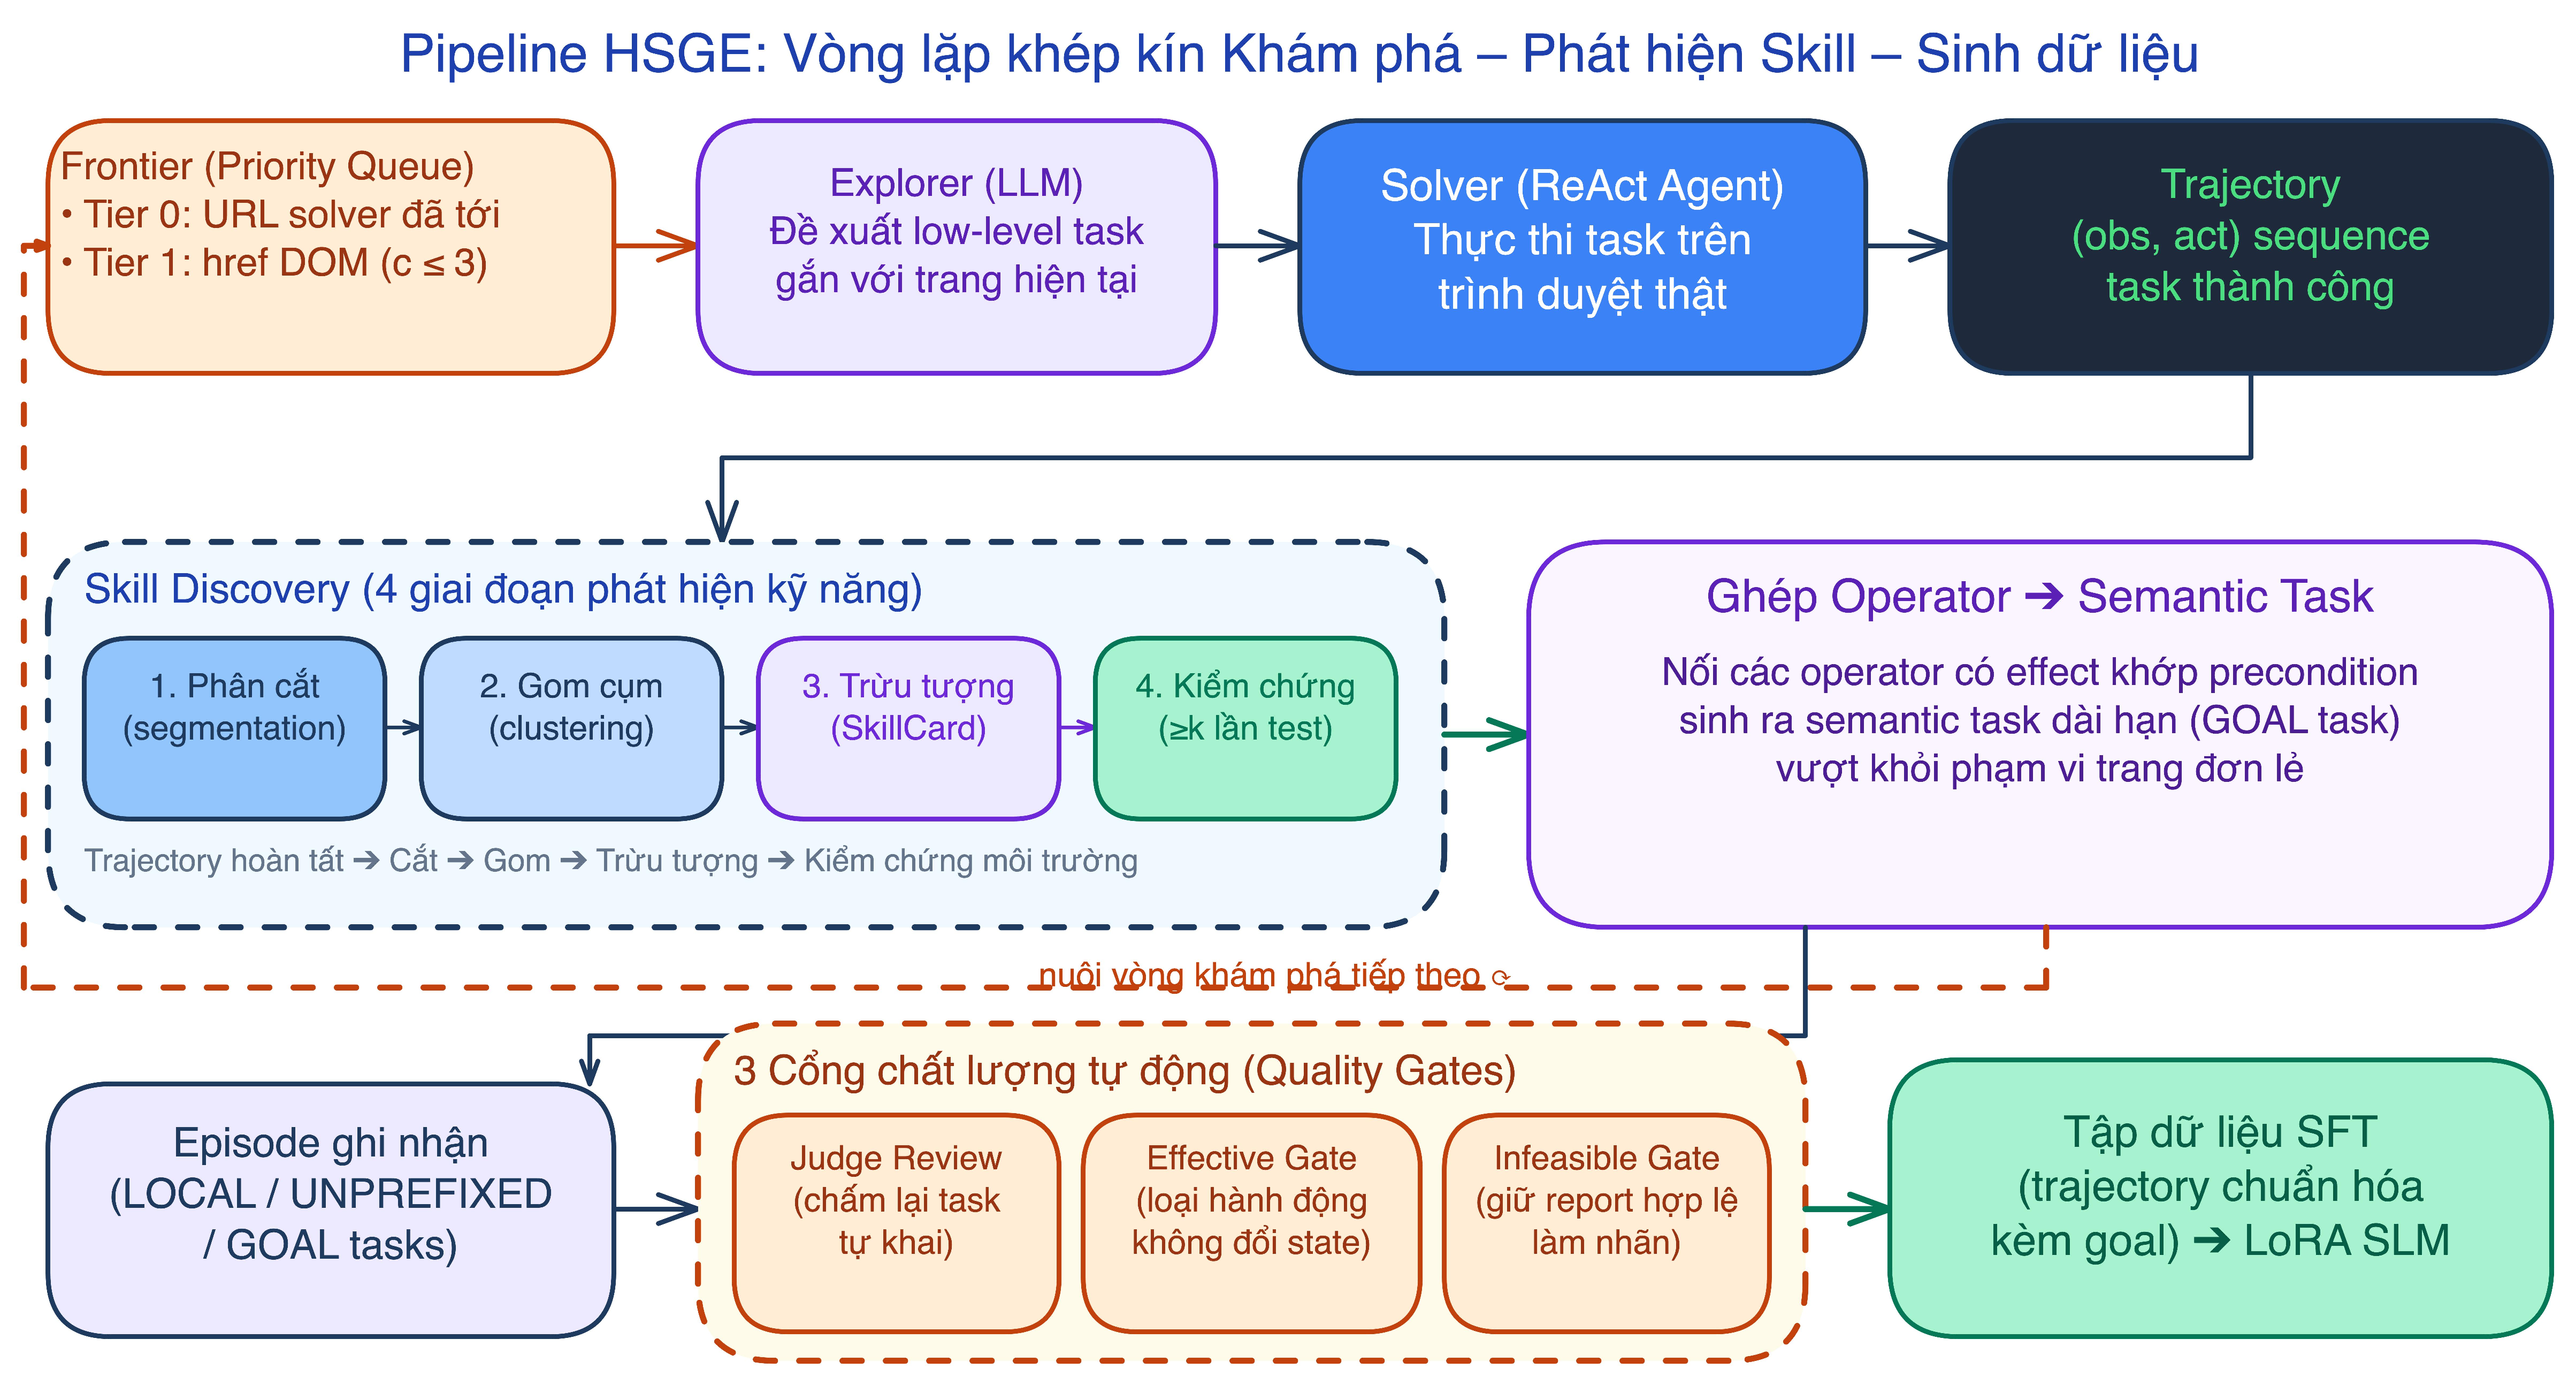
\includegraphics[width=\linewidth,height=0.62\textheight,keepaspectratio]{fig_pipeline.pdf}
  \end{center}
  \figcap{Vòng lặp khép kín: Khám phá $\rightarrow$ Phát hiện skill $\rightarrow$ Quy nạp operator $\rightarrow$ Ghép semantic task $\rightarrow$ Tinh lọc dữ liệu.}
\end{frame}

\subsection{Thiết lập \& phễu dữ liệu}
\begin{frame}{Thiết lập thực nghiệm và phễu dữ liệu thu được}
  \begin{columns}[t]
    \begin{column}{0.46\textwidth}
      \footnotesize
      \textbf{Thiết lập}
      \begin{itemize}\setlength{\itemsep}{3pt}
        \item \textbf{Môi trường}: 4 website WebArena tự triển khai (Shopping, Shopping Admin, GitLab, Reddit).
        \item \textbf{Khám phá}: 4 đợt ($\approx$21h/site), \kw{20\,808 lượt gọi LLM}.
        \item \textbf{Đánh giá}: \kw{655 task chính thức}, chấm tự động, 15 bước/task, \texttt{temperature}$=0$.
        \item \textbf{Huấn luyện}: Qwen3.5-9B $+$ LoRA, 1119 bước (5h09).
      \end{itemize}
    \end{column}
    \begin{column}{0.52\textwidth}
      \footnotesize
      \textbf{Phễu dữ liệu} (4 website)
      \vspace{0.03cm}

      \scriptsize
      \begin{tabular}{@{}L{4.2cm} R{1.4cm}@{}}
        \toprule
        Node đã duyệt (71 trùng lặp) & \textbf{455} \\
        Episode ghi nhận & \textbf{3981} \\
        Episode hợp lệ sau kiểm chứng & \textbf{2117} (53,2\%) \\
        \midrule
        Skill thu nhận / Operator quy nạp & \textbf{146 / 57} \\
        Semantic task sinh ra & \textbf{142} \\
        \midrule
        Trajectory vào dataset & \textbf{1760} \\
        Mẫu huấn luyện (Train/Val) & \textbf{8554 / 453} \\
        \bottomrule
      \end{tabular}
      {\scriptsize \kw{0} mục tiêu trùng train/val, \kw{0} nhãn từ con người. Chi phí API: \textbf{\$36,48}.}
    \end{column}
  \end{columns}
\end{frame}

\subsection{Phân tích \& diễn giải kết quả}
\begin{frame}{Kết quả chính trên 655 task và diễn giải}
  \centering
  \footnotesize
  \setlength{\tabcolsep}{4pt}
  \begin{table}
    \begin{tabular}{@{}L{2.6cm} R{2.5cm} R{2.5cm} R{1.6cm} R{2.0cm}@{}}
      \toprule
      \textbf{Website} & \textbf{Mô hình nền} & \textbf{Sau fine-tune} &
      \textbf{Chênh lệch} & \textbf{$p$ (McNemar)} \\
      \midrule
      Shopping       & 37/187 $=$ 19,8\% & 53/187 $=$ 28,3\% & $+$8,6  & 0,011 \\
      Reddit         & 7/106 $=$ 6,6\%   & 36/106 $=$ 34,0\% & $+$27,4 & $<$0,001 \\
      GitLab         & 20/180 $=$ 11,1\% & 33/180 $=$ 18,3\% & $+$7,2  & 0,011 \\
      Shopping Admin & 23/182 $=$ 12,6\% & 39/182 $=$ 21,4\% & $+$8,8  & 0,005 \\
      \midrule
      \textbf{Tổng} & \textbf{87/655 $=$ 13,3\%} & \textbf{161/655 $=$ 24,6\%} &
      \kw{$+$11,3\%} & \kw{$<$0,001} \\
      \bottomrule
    \end{tabular}
  \end{table}

  \vspace{0.1cm}
  \begin{columns}[t]
    \begin{column}{0.48\textwidth}
      \scriptsize
      \textbf{Đánh giá công bằng, nghiêm ngặt}: cùng tập task, prompt, ngân sách bước, bộ chấm. McNemar theo cặp: \kw{100 task} chỉ mô hình fine-tune giải được (vs 26 task mô hình nền).
    \end{column}
    \begin{column}{0.48\textwidth}
      \scriptsize
      \textbf{Diễn giải}: ý nghĩa thống kê trên \kw{toàn bộ 4/4 website} ($p \le 0{,}011$); lỗi định dạng đầu ra giảm từ 26,0\% xuống 0,6\% $\Rightarrow$ SLM làm chủ giao diện hành động.
    \end{column}
  \end{columns}
\end{frame}

\subsection{Minh họa thực thi (Demo)}
\begin{frame}{Demo: mô hình sau fine-tune giải một task WebArena}
  \begin{columns}[c]
    \begin{column}{0.42\textwidth}
      \footnotesize
      \textbf{Đặc điểm thực thi}
      \begin{itemize}\setlength{\itemsep}{4pt}
        \item \textbf{Đầu vào}: chỉ URL $+$ accessibility tree (không dùng ảnh).
        \item \textbf{Định dạng chuẩn}: sinh \texttt{thought} và \texttt{action} chuẩn xác.
        \item \textbf{Tự động chấm}: benchmark chính thức tự kiểm chứng hoàn thành task.
      \end{itemize}
    \end{column}
    \begin{column}{0.56\textwidth}
      \centering
      \setbeamercolor{demoframe}{bg=structure.fg!8,fg=structure.fg}
      \begin{beamercolorbox}[wd=\linewidth,ht=0.5\textheight,center]{demoframe}
        \vfill
        {\large \textbf{[\,DEMO TRỰC TIẾP / VIDEO\,]}}\\[0.3cm]
        {\footnotesize Chạy trực tiếp một vòng khám phá + giải task, hoặc video quay sẵn}
        \vfill
      \end{beamercolorbox}
    \end{column}
  \end{columns}
\end{frame}

% !TEX root = ../main.tex

%%% ============================================================
\section{Quá trình tạo và hoàn thiện báo cáo}
%%% ============================================================

\subsection{Năm giai đoạn viết báo cáo}
\begin{frame}{Báo cáo được viết như thế nào: 5 giai đoạn}
  \footnotesize
  Nhóm dùng hai công cụ AI với hai vai trò tách biệt: \textbf{một công cụ để viết}
  (brainstorm dàn ý, viết nháp, sửa file, build PDF) và \textbf{một công cụ khác để
  đọc lại và phản biện} bản vừa viết ra --- giống như nhờ một người khác đọc bản
  thảo thay vì tự mình vừa viết vừa tự chấm điểm cho chính mình. \textbf{Sinh viên
  là người quyết định} ở mọi bước: chọn giữ ý nào, bỏ ý nào, viết lại câu chữ cuối
  cùng bằng văn phong của mình.

  \vspace{0.15cm}
  \textbf{Ví dụ cụ thể — viết Chương 5 (Bàn luận)}:
  \begin{enumerate}\scriptsize\setlength{\itemsep}{2pt}
    \item \textbf{Dàn ý}: đưa cho công cụ viết bốn câu hỏi nghiên cứu (CH1--CH4) và
      số liệu thực nghiệm đã có $\rightarrow$ nó đề xuất dàn ý 3 mục; sinh viên chốt lại.
    \item \textbf{Viết nháp}: công cụ viết soạn từng mục theo dàn ý đã chốt, chỉ dùng
      số liệu có thật trong file kết quả, không được tự suy diễn con số.
    \item \textbf{Đọc lại phản biện}: công cụ đọc lại phát hiện mục CH4 chưa thực sự trả
      lời câu hỏi đặt ra ở Chương 1 $\rightarrow$ chỉ ra chỗ thiếu, đề xuất hướng bổ sung.
    \item \textbf{Sinh viên chỉnh sửa}: đọc góp ý, quyết định bổ sung đoạn nào, viết lại
      bằng lời văn của mình, rồi mới đưa công cụ viết sửa file \texttt{.tex}.
    \item \textbf{Build lại \& lưu}: build PDF kiểm tra không lỗi, rồi mới commit.
  \end{enumerate}
\end{frame}

\subsection{Vòng chỉnh sửa theo nhận xét của GVHD}
\begin{frame}{Một vòng chỉnh sửa diễn ra như thế nào}
  \begin{columns}[t]
    \begin{column}{0.52\textwidth}
      \footnotesize
      \textbf{Các bước, minh họa bằng một lần sửa thật}
      \begin{enumerate}\scriptsize\setlength{\itemsep}{2.5pt}
        \item GVHD nhận xét: "kết quả và bàn luận đang lẫn vào nhau, tách riêng ra".
        \item Đọc bản hiện tại cùng nhận xét đó, liệt kê những chỗ cụ thể cần sửa
          và xếp thứ tự quan trọng.
        \item Sửa từng chỗ trong file \texttt{.tex}, build lại PDF sau mỗi lần sửa
          để kiểm tra ngay, không dồn hết vào cuối.
        \item Đọc lại lần hai: \textbf{xác nhận trước} chỗ nào đã ổn, rồi mới nêu
          thêm điều còn thiếu, chia theo mức độ ưu tiên.
        \item Còn điểm cần sửa thì quay lại bước 3; khi ổn thì gửi lại cho GVHD.
      \end{enumerate}
    \end{column}
    \begin{column}{0.44\textwidth}
      \begin{alertblock}{Những gì luôn được kiểm tra lại}
        \footnotesize
        \begin{itemize}\setlength{\itemsep}{2.5pt}
          \item \textbf{Trích dẫn}: mỗi nguồn được tra lại trên Google Scholar/DOI;
            không tìm thấy, hoặc bài báo không nói đúng điều đang trích, thì bỏ hoặc sửa lại.
          \item \textbf{Số liệu}: mọi con số trong báo cáo chỉ lấy từ kết quả chạy
            thực tế, không được bịa hay chỉnh sửa cho đẹp.
          \item \textbf{Vai trò của AI}: AI chỉ là công cụ hỗ trợ, không phải đồng
            tác giả; sinh viên chịu trách nhiệm toàn bộ nội dung.
        \end{itemize}
      \end{alertblock}
      {\scriptsize Trước mỗi lần nộp: build lại toàn bộ, đảm bảo không còn lỗi biên dịch hay tham chiếu thiếu.}
    \end{column}
  \end{columns}
\end{frame}

% !TEX root = ../main.tex

%%% ============================================================
\section{Trả lời các câu hỏi phản biện}
%%% ============================================================

\subsection{Tính hợp lệ của phép đánh giá}
\begin{frame}{Khám phá và đánh giá trên cùng website --- có hợp lệ không?}
  \footnotesize
  \begin{columns}[t]
    \begin{column}{0.49\textwidth}
      \textbf{Cái \emph{không} xảy ra --- ranh giới train/test}
      \scriptsize
      \begin{itemize}\setlength{\itemsep}{2pt}
        \item Pipeline \kw{chưa từng nhìn thấy} 655 task của benchmark --- task huấn
              luyện do agent tự đề xuất từ giao diện.
        \item CSDL được \kw{khôi phục nguyên bản} trước mỗi đợt đo.
        \item Không trajectory thu thập nào được dùng lại lúc chấm.
      \end{itemize}
      \vspace{0.04cm}
      \textbf{Cái \emph{có} xảy ra --- và là chủ ý}
      \scriptsize
      \begin{itemize}\setlength{\itemsep}{2pt}
        \item Huấn luyện và đánh giá trên \emph{cùng} website --- đây là
              \kw{giao thức chuẩn} của cả dòng nghiên cứu: Go-Browse khám phá 20 URL
              mỗi domain của WebArena rồi chấm trên chính 812 task WebArena.
      \end{itemize}
    \end{column}
    \begin{column}{0.49\textwidth}
      \textbf{Vì sao không đo trên ``app khác cùng lĩnh vực''?}
      \scriptsize
      \begin{itemize}\setlength{\itemsep}{2pt}
        \item Đó là một bài toán \emph{khác}: tổng quát hóa ngoài miền --- và số liệu
              cho thấy \kw{chưa ai giải được}. Trên Online-Mind2Web (web mở):
        \end{itemize}
      \vspace{-0.05cm}
      \centering
      \begin{tabular}{@{}L{3.1cm} R{1.3cm}@{}}
        \toprule
        \textbf{Mô hình} & \textbf{SR} \\
        \midrule
        NNetNav-7B & 4,00\% \\
        Go-Browse-7B (SOTA ${<}10$B) & 5,33\% \\
        GPT-4o-mini & 9,33\% \\
        \bottomrule
      \end{tabular}\par
      \vspace{0.08cm}
      \raggedright
      \scriptsize Hai hệ thống chuyên biệt hóa trong miền đều \emph{thua} GPT-4o-mini
      khi ra web mở.
    \end{column}
  \end{columns}
  \vspace{0.1cm}
  {\scriptsize\textbf{Phát biểu đúng phạm vi.} Khóa luận \kw{không} tuyên bố mô hình
  tổng quát sang website chưa từng thấy --- đã ghi rõ ở mục ``Hợp lệ ngoại vi''. Và nếu
  phản đối ``cùng app thì không hợp lệ'' đứng vững, nó bác bỏ luôn Go-Browse lẫn
  NNetNav --- toàn bộ đường cơ sở để so sánh.\par}
\end{frame}

\subsection{Định vị: tổng quát ở đâu?}
\begin{frame}{Hướng đến ai --- và thứ gì mới là thứ tổng quát}
  \footnotesize
  \begin{columns}[t]
    \begin{column}{0.5\textwidth}
      \textbf{Người dùng đích}
      \scriptsize
      \begin{itemize}\setlength{\itemsep}{2pt}
        \item Nhóm/doanh nghiệp vận hành \kw{một số website cố định} --- trang quản
              trị nội bộ, CMS, diễn đàn riêng --- muốn một agent chạy tại chỗ.
        \item Họ không cần một agent ``biết mọi trang thương mại điện tử''. Họ cần một
              agent \emph{thạo đúng trang của họ}, rẻ và không gửi dữ liệu ra ngoài.
      \end{itemize}
      \vspace{0.12cm}
      \begin{block}{Câu chốt}
        \scriptsize
        Thứ tổng quát hóa là \kw{pipeline}, không phải \kw{model}. Model là sản phẩm
        dùng cho \emph{một} website; pipeline mới là đóng góp tái sử dụng được cho
        website tiếp theo.
      \end{block}
    \end{column}
    \begin{column}{0.48\textwidth}
      \textbf{Vì sao định vị này là khả thi về kinh tế}
      \scriptsize
      \vspace{0.05cm}
      \begin{tabular}{@{}L{3.4cm} R{1.5cm}@{}}
        \toprule
        Chi phí API (4 website) & \$54,21 \\
        Chi phí GPU (fine-tune + đánh giá) & \$24,40 \\
        \midrule
        \textbf{Cả chu trình} & \textbf{\$78,61} \\
        \textbf{Trung bình mỗi website} & \kw{$<$ \$20} \\
        \bottomrule
      \end{tabular}\par
      \vspace{0.1cm}
      \raggedright
      Đối chiếu: AutoWebGLM cần \kw{20 người gán nhãn làm một tháng} cho một tập
      $\approx$10.000 trajectory.
      \vspace{0.08cm}

      $\Rightarrow$ Ở mức dưới \$20 mỗi website và \kw{không cần người gán nhãn}, việc
      dựng một model riêng cho \emph{từng} website trở thành lựa chọn hợp lý hơn hẳn
      việc theo đuổi một model tổng quát.
    \end{column}
  \end{columns}
\end{frame}

\subsection{Kiểm soát chất lượng trong lúc thu thập}
\begin{frame}{Task có thật không, đủ bước không, và dựa vào đâu nói đã xong?}
  \scriptsize
  \begin{block}{1. Làm sao biết task LLM đề xuất là hợp lý và làm được trên giao diện đó?}
    Bộ đề xuất là một \emph{agent}, đọc trực tiếp cây trợ năng của trang thật và có thể
    thao tác thử trước khi đề xuất --- không đề xuất từ trí nhớ. Quan trọng hơn:
    \kw{tính khả thi được chứng minh bằng thực thi, không bằng lời}. Chỉ task có ít nhất
    một lượt giải \emph{thành công và qua kiểm chứng} mới vào dataset.
    $\Rightarrow$ 637 task bị chính agent báo bất khả thi; 3981 lượt thử chỉ còn
    \kw{2117 hợp lệ (53,2\%)}.
  \end{block}
  \vspace{-0.1cm}
  \begin{block}{2. Vì sao ngân sách 15 bước (task cục bộ) và 25 bước (semantic task)?}
    Solver chiếm \kw{85,5\%} trong 20.808 lượt gọi LLM, nên ngân sách bước \emph{chính
    là} ngân sách tiền --- đây trước hết là một quyết định chi phí. Nhưng dữ liệu cho
    thấy nó \kw{không bóp méo phép đo}: episode thành công có trung vị \kw{6 bước}
    (thất bại 13), và \kw{không episode nào} đạt được mục tiêu rồi mới bị cắt vì hết
    bước. Ngân sách đang đóng vai trò \emph{thước đo}, không phải \emph{hình phạt}.
  \end{block}
  \vspace{-0.1cm}
  \begin{block}{3. Dựa vào đâu để nói một task đã hoàn thành?}
    Ba lớp, mỗi lớp bắt loại lỗi lớp trước không thấy:
    \textbf{(i)} solver tự khai (\texttt{send\_msg\_to\_user}) hoặc vị từ tất định;
    \textbf{(ii)} \kw{LLM-as-Judge} soi lại trạng thái trang cuối $\rightarrow$ hạ cấp
    \kw{801 lượt} tự khai sai (27\%);
    \textbf{(iii)} cổng ``hành động hữu hiệu'' bằng mã, loại \kw{104 trajectory} tuyên
    bố xong mà không đổi gì trên trang --- nhóm lỗi mà judge \emph{về nguyên tắc} không
    thấy được, vì trang cuối không hề thay đổi.
    \vspace{0.04cm}

    \kw{Lưu ý}: đó là kiểm chứng lúc \emph{thu thập}. Còn con số 24,6\% được chấm bằng
    \kw{bộ chấm chính thức của WebArena}, không dùng judge của nhóm.
  \end{block}
\end{frame}

\subsection{Mục tiêu thực nghiệm và mức độ trả lời}
\begin{frame}{Thực nghiệm nhắm mục tiêu nào --- và đã trả lời tới đâu?}
  \scriptsize
  \setlength{\tabcolsep}{3pt}
  \renewcommand{\arraystretch}{1.15}
  \begin{tabular}{@{}L{0.9cm} L{4.5cm} L{4.9cm} L{1.5cm}@{}}
    \toprule
    \textbf{Câu hỏi} & \textbf{Số liệu} & \textbf{Kết quả} & \textbf{Trạng thái} \\
    \midrule
    \textbf{CH1} & 455 trang; 3981 lượt thử; 146 skill / 57 operator &
    1760 trajectory $\rightarrow$ 8554 mẫu; \$54,21 (0,0308\$/traj) & \kw{Đạt} \\
    \textbf{CH2} & 655 task, cùng prompt/ngân sách/bộ chấm; McNemar &
    13,3\% $\rightarrow$ 24,6\%; có ý nghĩa \emph{cả 4/4} website & \kw{Đạt} \\
    \textbf{CH3} & Tính lại các công trình trên đúng 4 website &
    Ngang Go-Browse-7B (2,0 $<$ CI $\pm$3,3); rẻ hơn 3,3$\times$ & \kw{Đạt} \\
    \textbf{CH4} & Phân loại lỗi; đo hiệu ứng bổ sung dữ liệu &
    85--96\% lỗi thực thi; gấp 3 dữ liệu chỉ $+$2,1 đpt & \kw{Đạt phần chẩn đoán} \\
    \bottomrule
  \end{tabular}

  \vspace{0.12cm}
  \begin{alertblock}{Phần thành thật phải nói kèm}
    \scriptsize
    \textbf{O2} hoàn thành một phần: chỉ 12/142 semantic task đến từ ghép chuỗi
    operator, phần còn lại từ seed năng lực website. \textbf{O4} hoàn thành một phần:
    mỗi task mới đo \emph{một} lần, và \kw{ablation đồ thị so với khám phá phẳng ---
    phép đo duy nhất chứng minh trực tiếp giá trị của cấu trúc đồ thị --- vẫn chưa chạy}.
  \end{alertblock}
\end{frame}


\begin{frame}[plain]
  \centering
  \vfill
  {\usebeamerfont{title}\color{structure.fg}\Large\textbf{XIN CẢM ƠN THẦY/CÔ}}\\[0.3cm]
  {\normalsize Nhóm rất mong nhận được góp ý để hoàn thiện báo cáo trước khi bảo vệ}
  \vfill
  \footnotesize
  \begin{tabular}{ll}
    \textbf{Sinh viên thực hiện:} & Trương Bảo Kiệt (22127223) --- Hồ Tiến Phát (22127321) \\
    \textbf{GVHD:} & PGS.TS. Nguyễn Văn Vũ \\
    \textbf{Đơn vị:} & Bộ môn CNPM, Khoa CNTT --- Trường ĐH KHTN, ĐHQG-HCM
  \end{tabular}
  \vfill
\end{frame}

\end{document}
